
%(BEGIN_QUESTION)
% Copyright 2006, Tony R. Kuphaldt, released under the Creative Commons Attribution License (v 1.0)
% This means you may do almost anything with this work of mine, so long as you give me proper credit

In this density measurement system, what will the output of the transmitter be when the vessel is filled with clean water?

$$\includegraphics[width=15.5cm]{i00284x01.eps}$$

What will the output of the transmitter be when the vessel is filled with carbon tetrachloride (D = 99.573 lb/ft$^{3}$)?

\vskip 10pt

Finally, specify the density measurement range in units of {\it specific gravity}.

\underbar{file i00284}
%(END_QUESTION)





%(BEGIN_ANSWER)

When the vessel is holding clean water, the transmitter output will be 4 mA.

\vskip 10pt

When the vessel is holding carbon tetrachloride, the transmitter output will be 13.52 mA.

\vskip 10pt

LRV = 1.0 ; URV = 2.0 (specific gravity)

%(END_ANSWER)





%(BEGIN_NOTES)


%INDEX% Measurement, density: bubble tube (bubbler)
%INDEX% Measurement, density: dip tube (bubbler)

%(END_NOTES)


